Often, energy available at the transiently-powered device is sufficient to run multiple consecutive tasks without page commit at each task boundary. In this case task-based execution model can better amortize the run time overhead of committing updated pages when a task ends. Hence many tasks can be \emph{merged} into a single virtual task---a process we call \emph{coalescing}. 

\textbf{Process of Task Coalescing.} \sys, as the first task-based execution model, dynamically coalesces consecutively executing tasks at run time. When $X$ tasks are coalesced, the $X-1$ tasks do not commit their updates to protected memory locations when reaching a \transition statement. Instead, execution immediately continues from the beginning of the $X$th task. At the end of the $X$th coalesced task, \sys commits the pages that were updated by any of the $X$ coalescing tasks. If consecutive tasks access the same pages of data, the pages accessed by both tasks only need to be committed once. \sys repeatedly executes $X-1$ coalesced tasks, followed by a committing task. 

\textbf{Coalescing Speed/Wasted Effort Trade-off.} \sys can coalesce an arbitrary number of consecutive tasks. As more tasks coalesce, their collective commit overhead amortizes better, potentially improving performance. However, as more tasks coalesce, the amount of potentially {\em wasted work} also increases. If power fails during a long sequence of coalesced tasks the lack of an intervening commit requires execution to restart from the {\em first} task in the sequence, failing to preserve the progress of any of the tasks in this long sequence. The challenge to coalescing tasks is determining how many tasks to coalesce before committing. During execution, an executing task is either a {\em coalesced} task, which does not commit its state before transitioning or a {\em committing} task, which does commit its state before transitioning.

\textbf{Task Coalescing Strategies.} The simplest strategy will coalesce/de-coalesce fixed number of task at every successful/unsuccessful commit operation, where task coalescing factor increases by $C_U$ at each successful virtual task execution and decreases by $C_D$, otherwise. There are naturally infinite possible strategies for coalescing, i.e. infinite amount of $(C_U,C_D)$ pairs. The caveat of predefined $(C_U,C_D)$ pair is inability to adapt to changing energy availability conditions. A \emph{good} coalescing strategy must moderates the risk of coalescing and capitalize on its benefit by dynamically, \emph{adaptively} determining a coalescing factors $(C_U,C_D)$ that combines many tasks without suffering an excess of wasted work. Therefore we propose to consider two fundamental coalescing strategies for \sys, which we will later assess and compare experimentally:

\begin{enumerate}
	\item \textbf{Power Interrupt History-based Coalescing (HDC):} when more tasks are coalesced without power interrupt $C_U$ increases gradually, and $C_D$ increases, as more task are interrupted before committing; and 
	\item \textbf{Weighted Power Interrupt History-based Coalescing (WHDC):} where coalescing strategy follows the one of HDC, while also taking into account the \emph{expected execution time} of each task in the application.
\end{enumerate}

\subsection{Power Interrupt History-driven Coalescing}

With this strategy \sys calculates only one parameter $C=C_U=C_D$ based on the number of tasks completed, until $t$th task commit, $S_t$, during the current operational period. \sys begins execution in a coalesced task with $S_t=0$. When $S_t=C_{t-1}-1$ coalesced tasks have been executed without power interrupt (where $C_{t-1}$ defines $C$ until $t-1$ task commit) a task commit follows. After each commit, \sys assigns new coalescing factor as $C_{t}=\lceil \sum_{k=1}^{t}S_{k-1}/2\rceil$. This implies that if more tasks complete in an operating period, \sys attempts to coalesce more tasks. However, tasks coalescing are increased by a half the speed of the successful task completion. This way we adapt to the coalescing speed/wasted effort trade-off: at the potential power interrupt. In the power failure case, if fewer tasks complete, \sys attempts to coalesce fewer tasks.

%\textbf{Task Coalescing Illustration.} Figure~\ref{fig:coalescing_example_states} shows a sequence of three tasks executing in \sys. At left, there is no coalescing and tasks incur the cost of commit at each transition. The center shows the same tasks executing as coalesced groups of two tasks $C=2$, avoiding one commit. At right, \sys coalesces three tasks ($C=3$) avoiding two commits. Figure~\ref{fig:coalescing_example_flowchart} shows how \sys adapts the value of $C$ based on $S$. \sys executes tasks in the first operating period, with $C$ equal to half the number of tasks completed in the prior execution period. In the example, $C$ starts at eight. After completing eight tasks, \sys commits and reduces $C$ by half to four. \sys completes two of four tasks and power fails.  During the operating period, \sys executed a total of ten tasks (i.e., $S=10$) and when \sys restarts, $C$ is assigned to five (i.e., half of $S$). \sys completes the five coalesced tasks $S=5$ and after committing, assigns $C$ to half of $S$, which is three (after rounding up). \sys coalesces three tasks and again commits.  At this point, $S=8$; \sys assigns $C=4$ and execution continues.

\subsection{Weighted Power Interrupt History-driven Coalescing}

The previous coalescing strategy is oblivious to the task size. Although many tasks can be coalesced, their non-equal size will determine that some coalesced tasks will be more susceptible to power interrupts than others. To understand that effect we provide the following illustration. 

\textbf{Task Size Profiling.} To measure how large the distribution of tasks is, we have used a set of program benchmarks (refer to Section~\ref{sec:results_software} for details and to the beginnin of Section~\ref{sec:methodology_evaluation} for system setup). Each benchmark was run for predefined period of time (X\,seconds \todo{Provide exact number}{Amjad}), on non-intermittent power, and at each task evocation, its execution time was measured. If a task was evoked more than once, longer execution time replaced the short one---this way we obtained conservative values of task sizes. At the end of task measurement, normalized values of task execution are assigned for each task, the shortest one being one task, the longest one X tasks \todo{Provide exact number}{Amjad}. Result of the task size measurement is provided in Figure~\ref{fig:task_profiling}. We observe huge variations of task sizes---both within a benchmark, as well per benchmark, which calls for the use of this information in coalescing.

\begin{figure}
	\centering
	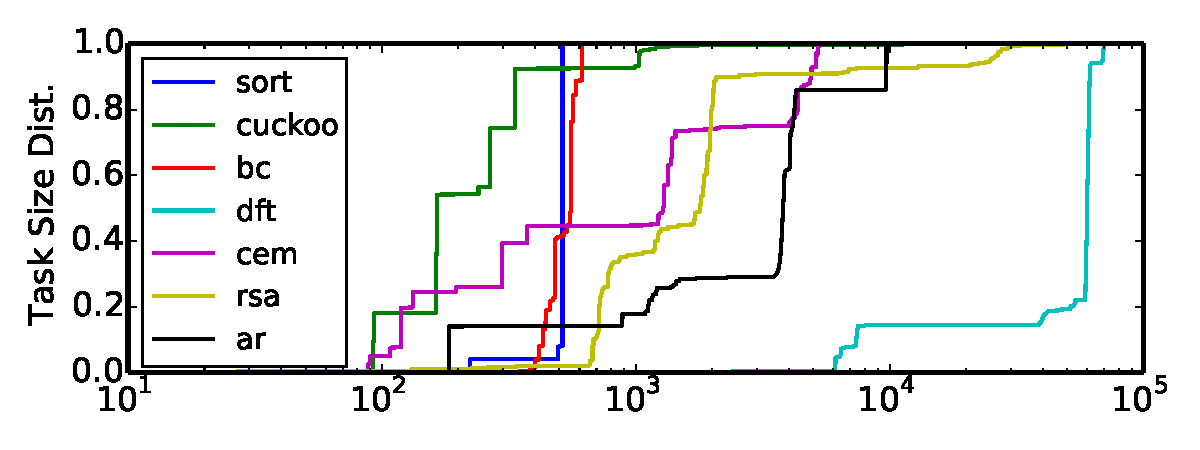
\includegraphics[width=\columnwidth]{figures/TskDist.pdf}%coalescing_timeline
	\caption{Result of benchmark applications (Section~\ref{sec:results_software}) task size measurement, measured in the number of instruction cycles. We observe very large variations of task sizes per each benchmark. \todo{Describe X axis, no capitals in titles - except first word; markers in addition to colors per app; remove 4.7}{Amjad}}
	\label{fig:task_profiling}
\end{figure}

In the second coalescing strategy an application needs to be profiled, as above, before it is loaded to the intermittently-powered device.

%\begin{figure}
%	\centering
	%\subfloat[\sys coalesces consecutive tasks.]{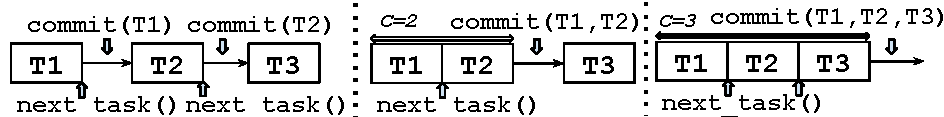
\includegraphics[width=\columnwidth]{figures/coalescing_states}\label{fig:coalescing_example_states}}\\
	%\subfloat[\sys dynamically adapts the amount of coalescing.]{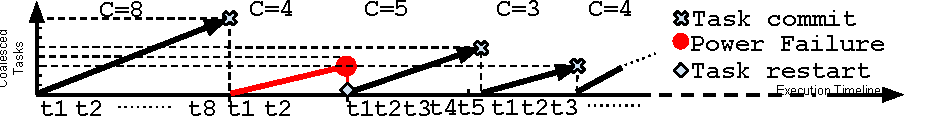
\includegraphics[width=\columnwidth]{figures/coalescing_timeline}\label{fig:coalescing_example_flowchart}}
	%\caption{\sys coalesces tasks to avoid overheads.}
	%\label{fig:coalescing_example}
%\end{figure}

%However, it takes a conservative approach by making the virtual task size equal
%to the half of the number of successfully executed real tasks before the last
%power interrupt (see lines~\ref{algo:coalescing:executionHistory1},
%\ref{algo:coalescing:executionHistory2} of Algorithm~\ref{algo:coalescing}). 
%
%We
%advocate for the algorithm conservative approach by the following two reasons:
%(i) the power interrupts are not uniformly distributed over the tasks; and (ii)
%the re-execution penalty, in case of a power interrupt, grows linearly with the
%size of a virtual task. 
%
%Furthermore, the algorithm considers the charging rate
%by allowing the real tasks counter (RTC), which represents the execution
%history between the last two power interrupts, to increase from one up to
%multiple virtual tasks (see line~\ref{algo:coalescing:realTaskCounter} of
%Algorithm~\ref{algo:coalescing}). 
%
%As a consequence, the virtual task size
%changes rapidly (since it is half of the execution history) in response to the
%change in the charging rate. 
%
%However, the algorithm sets a limit to the size of
%the virtual task for these two reasons: (i) having an infinity virtual task
%size, results in a certain computation progress loss; and (ii) the benefit of
%task merging is governed by the diminishing return principle (which will be
%demonstrated experimentally in Section~\ref{sec:results_coalescing}).
%
%The algorithm protects itself from power interrupts by going into three stages:
%(i) virtual progressing, where the operations are done on the volatile memory
%(see
%lines~\ref{algo:coalescing:virtualProgressing1}--\ref{algo:coalescing:virtualProgressing2}
%of Algorithm~\ref{algo:coalescing} ); 
%(ii) transition stage, where the volatile
%state is moved to a temporary persistent buffer. 
%
%Until the end of the second
%stage if a power is interrupted, then all the virtual progress will be
%cancelled and the virtual task will re-executed and re-initialized from a
%consistent input (see line~\ref{algo:coalescing:virtualProgressing1} of
%Algorithm~\ref{algo:coalescing}); 
%
%and (iii) persistent commit stage, upon
%entering this stage the algorithm will make a firm transition (see
%lines~\ref{algo:coalescing:firmTransition1},
%\ref{algo:coalescing:firmTransition2} of Algorithm~\ref{algo:coalescing}) and
%it will not go back to the other stages unless all the data is committed from
%the persistent buffer to non-volatile memory. 
%
%Since the data is being moved in one direction and from a persistent location,
%power interrupt is tolerable at this stage. 

%\begin{algorithm}[t]
%	\caption{\sys task coalescing mechanism}
%	\label{algo:coalescing}
%	\scriptsize
%	\begin{algorithmic}[1]
%		\State $\text{p}$  \Comment{Indicates persistent variables, initialized \textbf{only} during device programming}
%		\State $\text{RT} \in \{\sys~\text{static tasks}\}$  \Comment{Real task}
%		\State $\text{VT} \subset \{~\text{RT's}\}$  \Comment{Virtual task}
%		\State $\text{RTC}$  \Comment{RT counter}
%		\State $\text{VTC}$  \Comment{VT counter}
%		% \State $|\text{VT}|$ \Comment{VT size measured in RT}
%		\State $\text{TVT}$ \Comment{Temporary VT}
%		\State $\text{VT}_{\max}$ \Comment{Maximum VT size measured in RT (coalescing upper bound)}
%		\vspace{0.1cm}
%		
%		\State $\text{p RTC} = x $ 
%		\State $\text{p VT}_{\max} = y$
%		\State $\text{p VT} = \text{RT}$ 
%		\State $\text{p TVT} = \text{VT} $ 
%		\State $\text{VTC} = 0 $ 
%		\vspace{0.1cm}
%
%		\Function{scheduler}{\null}
%
%			\State $\text{VTC} = \text{RTC/2} $  \label{algo:coalescing:executionHistory1}
%			\State $\text{RTC} = 0 $
%			\State $\text{RT} = \text{VT}$ \Comment{Recover virtual state} \label{algo:coalescing:virtualProgressing1}
%			\If{commiting}
%				\State $\text{RT}=\text{TVT}$
%				\State $\texttt{goto} \ \ \ref{commitStage}$ \label{algo:coalescing:firmTransition1}
%			\EndIf
%			\vspace{0.1cm}
%
%			\While {True}
%				\While{$\text{VTC}--$}
%					\Function{execute}{$\text{RT}$}
%					\EndFunction
%					\If{$\text{RTC} < \text{VT}_{\max}$}
%						\State $\text{RTC}++$  \label{algo:coalescing:realTaskCounter}
%					\EndIf
%					\State $\text{RT} \leftarrow \text{RT}_{next}$ \Comment{Virtual progressing}
%				\EndWhile        \label{algo:coalescing:virtualProgressing2}
%
%				\State \Comment{Virtual task is finished}
%				\State $\text{Data} \rightarrow \text{pTempBuf}$ \Comment{pTempBuf: persistent temporary buffer}
%				\State $\text{TVT} = \text{RT}$ 
%				\State $\text{commiting} = \text{True}$ \label{algo:coalescing:firmTransition2}
%				\State 
%				\State $\text{VT} = \text{TVT}$ \label{commitStage}
%				\State $\text{pTempBuf} \rightarrow \text{FRAM}$ 
%				\State $\text{VTC} = \text{RTC/2}$ 		\Comment{Set VT size} \label{algo:coalescing:executionHistory2}
%				\State $\text{commiting} = \text{False}$ 
%
%			\EndWhile
%
%		\EndFunction
%			
%	\end{algorithmic}
%\end{algorithm}

%\subsection{Power Interrupt Immune Scheduler}
%
%% TNT :  Total Number of Tasks
% JT 	: Total Jump
% ID	: Task ID
% D	: relative Jump (Delta)
% VCT_PT : Current Task Pointer

% if(TJ < TNT)
% 	VCT_PT <- VCT_PT + D
% else
% 	while ((dis = TJ - TNT) > TNT)
% 		dis -= ID
% 	VCT_PT <- VCT_PT + dis


\begin{algorithm}[t]
	\caption{\sys's scheduler: relative jump algorithm}
	\label{algo:relativeJump}
	\scriptsize
	%\small
	\begin{algorithmic}[1]
			\State \textsf{TNT}: Total Number of Tasks
			\State \textsf{ID}: Task ID
			\State \textsf{$\delta$}: Relative Jump
			\State $\textsf{TJ} \leftarrow (\textsf{ID} + \delta )$ \Comment{Total Jump}
			\State \textsf{\textsf{$VCT_{pt}$}}: Virtual Current Task Pointer

			\If { \textsf{TJ} > \textsf{TNT} }
				\State $\textsf{dis} = \textsf{TJ} - \textsf{TNT}$
				\While{ $ \textsf{dis} > TNT $ }
					\State $\textsf{dis} -= \textsf{TNT}$
				\EndWhile
				\State $\textsf{dis} -= \textsf{ID}$
				\State \textsf{$VCT_{pt}$} $+= \textsf{dis}$
			\Else
				\State \textsf{$VCT_{pt}$} $+= \delta $

			\EndIf
	\end{algorithmic}
\end{algorithm} %Task jumping algorithm
%
%It utilizes a persistent circular buffer (i.e. persistent linked list) to keep the state of a program across power failures. \sys provides an API to enable a programmer to have a full control over the execution flow of the program, i.e. (un)blocking a task or re-execute the same task which is particularly important in the intermittent execution to emulate a persistent loop. \todo{Expand this section}{Amjad}
%
%\begin{algorithm}
%	\caption{Opportunistic virtual Task size}
%	\label{algo:fixVirtTask}
%	\scriptsize
%	%\small
%	\begin{algorithmic}[1]
%		\State $VT \subset \text{\{\sys Tasks\}} $  \Comment{$VT:$ Virtual Task}
%		\State VTS : VT size
%		\vspace{0.1cm}
%		
%		\While {$True$}
%		\State $VT \leftarrow VT_{next}$
%		\vspace{0.1cm}
%		\While {execute $VT$} 
%		\If { $\text{power failed twice}$ }				
%		\State $VTS--$  
%		\EndIf
%		\EndWhile
%		
%		\vspace{0.1cm}
%		\If {$ \text{All tasks executed}$}
%		\State $VTS++$
%		\EndIf
%		\EndWhile
%	\end{algorithmic}
%\end{algorithm}
